\documentclass[aspectratio=169,11pt]{beamer}

\usepackage[T1]{fontenc}
\usepackage[utf8]{inputenc}
\usepackage{tikz}
\usepackage{booktabs}
\usepackage{xcolor}
\usepackage{helvet}
\renewcommand{\familydefault}{\sfdefault}

\usetikzlibrary{arrows.meta,positioning,calc,patterns,fit,shapes.geometric,backgrounds}

\usetheme{default}
\setbeamertemplate{navigation symbols}{}
\setbeamertemplate{footline}[frame number]
\setbeamercolor{background canvas}{bg=white}
\setbeamercolor{frametitle}{fg=black,bg=white}
\setbeamercolor{normal text}{fg=black}
\setbeamercolor{structure}{fg=black}
\setbeamerfont{frametitle}{series=\bfseries,size=\Large}

% Palette — clear, not purple-AI
\definecolor{ink}{HTML}{1A1A1A}
\definecolor{mute}{HTML}{5C5C5C}
\definecolor{line}{HTML}{D9D9D9}
\definecolor{c1}{HTML}{0B6E4F}   % multi-D green
\definecolor{c2}{HTML}{C45C26}   % IK orange
\definecolor{c3}{HTML}{1B4F72}   % orth blue
\definecolor{c4}{HTML}{6C3483}   % shooting purple-ish but muted plum
\definecolor{good}{HTML}{1E7A46}
\definecolor{bad}{HTML}{A93226}
\definecolor{kai}{HTML}{E67E22}
\definecolor{pedro}{HTML}{2980B9}
\definecolor{mario}{HTML}{27AE60}
\definecolor{bhuvi}{HTML}{8E44AD}
\definecolor{p5}{HTML}{7F8C8D}

\newcommand{\pill}[2]{%
  \tikz[baseline=(t.base)]{
    \node[fill=#1,text=white,font=\scriptsize\bfseries,
          inner xsep=5pt,inner ysep=2pt,rounded corners=2pt] (t) {#2};
  }%
}

% Horizontal fit bars: name, score/10, color
\newcommand{\fitbar}[3]{%
  \begin{tikzpicture}[baseline]
    \node[anchor=east,font=\scriptsize\bfseries,text=#3,
          minimum width=1.15cm,align=right,inner sep=0] at (0,0) {#1};
    \fill[line] (0.12,-0.11) rectangle (3.52,0.11);
    \fill[#3] (0.12,-0.11) rectangle ({0.12+0.34*#2},0.11);
    \node[anchor=west,font=\scriptsize,text=mute] at (3.6,0) {#2};
  \end{tikzpicture}%
}

\newcommand{\fitpanel}[5]{%
  \begin{tabular}{@{}l@{}}
    \fitbar{Kai}{#1}{kai}\\[2pt]
    \fitbar{Pedro}{#2}{pedro}\\[2pt]
    \fitbar{Mario}{#3}{mario}\\[2pt]
    \fitbar{Bhuvi}{#4}{bhuvi}\\[2pt]
    \fitbar{P5*}{#5}{p5}
  \end{tabular}%
}

\title{Numerical Methods --- Pick our project}
\author{Group of 5}
\date{Shortlist from the intake survey}

\begin{document}

%---------------------------------------------------------------------
\begin{frame}[plain]

\begin{tikzpicture}[remember picture,overlay]
  \fill[ink] (current page.south west) rectangle (current page.north east);
  \fill[c1] (0,0) rectangle (0.35\paperwidth,\paperheight);
  \node[anchor=west,text=white,font=\Huge\bfseries,align=left]
    at ([xshift=1.1cm,yshift=1.2cm]current page.west)
    {4 project ideas.\\[0.3em]
     \large One vote.};
  \node[anchor=west,text=white!70,font=\large,align=left]
    at ([xshift=1.1cm,yshift=-0.9cm]current page.west)
    {Built from your survey + course brief.\\
     Oral Q\&A = 70\% of the grade --- keep it explainable.};
  \node[anchor=south west,text=white!50,font=\small]
    at ([xshift=1.1cm,yshift=0.6cm]current page.south west)
    {P5* = 5th member (no survey yet) --- assumed flexible, syllabus-only};
\end{tikzpicture}
\end{frame}

%---------------------------------------------------------------------
\begin{frame}{How to read the next slides}
\begin{columns}[T]
\begin{column}{0.55\textwidth}
  \textbf{Each idea gets one slide:}\\[0.6em]
  {\color{c1}\rule{1.2em}{1.2em}}~~what it is\\[0.35em]
  {\color{c2}\rule{1.2em}{1.2em}}~~what we already know from class\\[0.35em]
  {\color{good}\rule{1.2em}{1.2em}}~~pros\quad
  {\color{bad}\rule{1.2em}{1.2em}}~~cons / who struggles\\[0.35em]
  {\color{mute}\rule{1.2em}{1.2em}}~~fit bars (0--10, from survey + roles)
\end{column}
\begin{column}{0.42\textwidth}
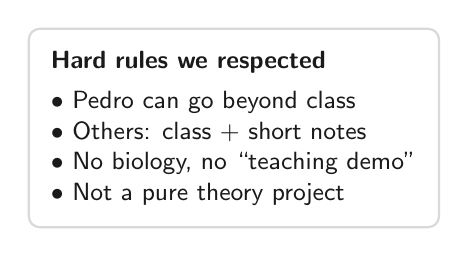
\begin{tikzpicture}
  \node[draw=line,thick,rounded corners=4pt,align=left,font=\small,
        inner sep=8pt,text=ink] {
    \textbf{Hard rules we respected}\\[0.4em]
    $\bullet$ Pedro can go beyond class\\
    $\bullet$ Others: class + short notes\\
    $\bullet$ No biology, no ``teaching demo''\\
    $\bullet$ Not a pure theory project
  };
\end{tikzpicture}
\end{column}
\end{columns}
\end{frame}

%---------------------------------------------------------------------
\begin{frame}{1 --- Multidimensional integrals for robot volumes}
\pill{c1}{BEST GROUP FIT}

\vspace{0.3em}
\begin{columns}[T]
\begin{column}{0.54\textwidth}
  \textbf{What}\\[0.2em]
  {\small Integrate in many variables. Compare grid methods vs random sampling. Apply to a robot-arm reachable volume.}\\[0.55em]

  \textbf{From class}\\[0.2em]
  {\small 1D Gauss / Simpson. Product rules in 2D+. Monte Carlo is on the project list (not lectured).}\\[0.55em]

  {\color{good}\textbf{+}} {\small Kai's favorite topic (10). Clear live plots. Pedro alone does sparse grids.}\\[0.25em]
  {\color{bad}\textbf{--}} {\small Kai dislikes leaning on Monte Carlo --- we keep it as baseline only.}
\end{column}
\begin{column}{0.44\textwidth}
  \fitpanel{10}{9}{8}{7}{7}

  \vspace{0.4em}
  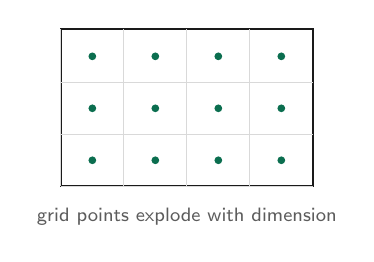
\begin{tikzpicture}
    % tiny visual: curse of dim
    \draw[thick,ink] (0,0) -- (3.2,0) -- (3.2,2.0) -- (0,2.0) -- cycle;
    \foreach \i in {0,...,3}
      \draw[line] ({\i*0.8},0) -- ({\i*0.8},2);
    \foreach \j in {0,...,2}
      \draw[line] (0,{\j*0.66}) -- (3.2,{\j*0.66});
    \foreach \i in {0,...,3}
      \foreach \j in {0,...,2}
        \fill[c1] ({\i*0.8+0.4},{\j*0.66+0.33}) circle (1.4pt);
    \node[font=\scriptsize,text=mute,anchor=north] at (1.6,-0.15) {grid points explode with dimension};
  \end{tikzpicture}
\end{column}
\end{columns}
\end{frame}

%---------------------------------------------------------------------
\begin{frame}{2 --- Quasi-Newton (BFGS) for robot arm aiming}
\pill{c2}{ROBOTICS DEMO}

\vspace{0.3em}
\begin{columns}[T]
\begin{column}{0.54\textwidth}
  \textbf{What}\\[0.2em]
  {\small Find joint angles so the arm tip hits a target. Compare gradient descent, Newton, and BFGS.}\\[0.55em]

  \textbf{From class}\\[0.2em]
  {\small Newton's method. Solving systems. Optimization is a suggested project topic.}\\[0.55em]

  {\color{good}\textbf{+}} {\small Cool animation. Pedro loves optimization (10). Mario/Kai strong on robotics/ML.}\\[0.25em]
  {\color{bad}\textbf{--}} {\small Bhuvi rated unconstrained opt only 3 --- needs a demo/Q\&A role, not theory.}
\end{column}
\begin{column}{0.44\textwidth}
  \fitpanel{8}{10}{8}{5}{7}

  \vspace{0.35em}
  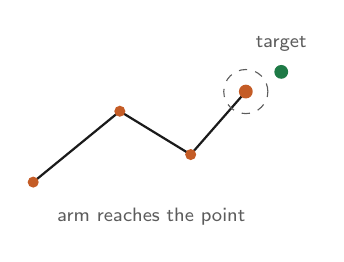
\begin{tikzpicture}
    \draw[thick,ink] (0,0) -- (1.1,0.9) -- (2.0,0.35) -- (2.7,1.15);
    \fill[c2] (0,0) circle (2pt);
    \fill[c2] (1.1,0.9) circle (2pt);
    \fill[c2] (2.0,0.35) circle (2pt);
    \fill[c2] (2.7,1.15) circle (2.5pt);
    \draw[dashed,mute] (2.7,1.15) circle (0.28);
    \fill[good] (3.15,1.4) circle (2.5pt);
    \node[font=\scriptsize,text=mute] at (3.15,1.75) {target};
    \node[font=\scriptsize,text=mute,anchor=north] at (1.5,-0.2) {arm reaches the point};
  \end{tikzpicture}
\end{column}
\end{columns}
\end{frame}

%---------------------------------------------------------------------
\begin{frame}{3 --- Orthogonal polynomials $\to$ Gaussian quadrature}
\pill{c3}{CLEAN MATH STORY}

\vspace{0.3em}
\begin{columns}[T]
\begin{column}{0.54\textwidth}
  \textbf{What}\\[0.2em]
  {\small Special polynomials that make integration very accurate. Compare to Simpson. Pedro alone extends to spectral methods for ODEs.}\\[0.55em]

  \textbf{From class}\\[0.2em]
  {\small Gaussian quadrature on the roadmap. Interpolation ideas. Suggested topic \#2.}\\[0.55em]

  {\color{good}\textbf{+}} {\small Everyone rated this $\ge 6$. Easy oral math. Member 5 stays fully in syllabus.}\\[0.25em]
  {\color{bad}\textbf{--}} {\small Less ``wow'' than a robot demo. Must not drift into minimax (Kai = 0).}
\end{column}
\begin{column}{0.44\textwidth}
  \fitpanel{9}{9}{7}{7}{8}

  \vspace{0.3em}
  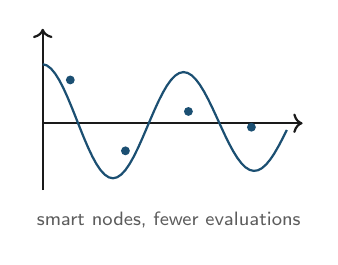
\begin{tikzpicture}
    \draw[->,thick,ink] (0,0) -- (3.3,0);
    \draw[->,thick,ink] (0,-0.85) -- (0,1.2);
    \draw[thick,c3,domain=0:3.1,samples=60]
      plot (\x, {0.75*cos(3.5*\x r)*exp(-0.08*\x)});
    \foreach \x/\y in {0.35/0.55, 1.05/-0.35, 1.85/0.15, 2.65/-0.05}
      \fill[c3] (\x,\y) circle (1.6pt);
    \node[font=\scriptsize,text=mute,anchor=north] at (1.6,-1.0) {smart nodes, fewer evaluations};
  \end{tikzpicture}
\end{column}
\end{columns}
\end{frame}

%---------------------------------------------------------------------
\begin{frame}{4 --- Shooting method: aim a trajectory}
\pill{c4}{CLASS IVP + ROOTFINDING}

\vspace{0.3em}
\begin{columns}[T]
\begin{column}{0.54\textwidth}
  \textbf{What}\\[0.2em]
  {\small Guess the launch angle, simulate the flight (RK), adjust until you hit the target. Optional: soft landing / multiple shooting (Pedro).}\\[0.55em]

  \textbf{From class}\\[0.2em]
  {\small Runge--Kutta + bisection/Newton. BVPs are on the syllabus but \emph{not} lectured --- explicit project green light.}\\[0.55em]

  {\color{good}\textbf{+}} {\small Live ``miss then hit'' demo. Reuses class tools. Strong robotics/physics interest.}\\[0.25em]
  {\color{bad}\textbf{--}} {\small Bhuvi low on BVP/IVP scores --- give them the demo, not the theory.}
\end{column}
\begin{column}{0.44\textwidth}
  \fitpanel{8}{9}{8}{5}{7}

  \vspace{0.25em}
  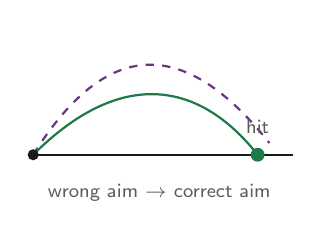
\begin{tikzpicture}
    \draw[thick,ink] (0,0) -- (3.3,0);
    \draw[thick,c4,dashed] (0,0) .. controls (1.0,1.6) and (2.0,1.4) .. (3.0,0.15);
    \draw[thick,good] (0,0) .. controls (1.1,1.1) and (2.1,0.95) .. (2.85,0);
    \fill[ink] (0,0) circle (2pt);
    \fill[good] (2.85,0) circle (2.5pt);
    \node[font=\scriptsize,text=mute] at (2.85,0.35) {hit};
    \node[font=\scriptsize,text=mute,anchor=north] at (1.6,-0.25) {wrong aim $\to$ correct aim};
  \end{tikzpicture}
\end{column}
\end{columns}
\end{frame}

%---------------------------------------------------------------------
\begin{frame}{Side-by-side fit}
\centering
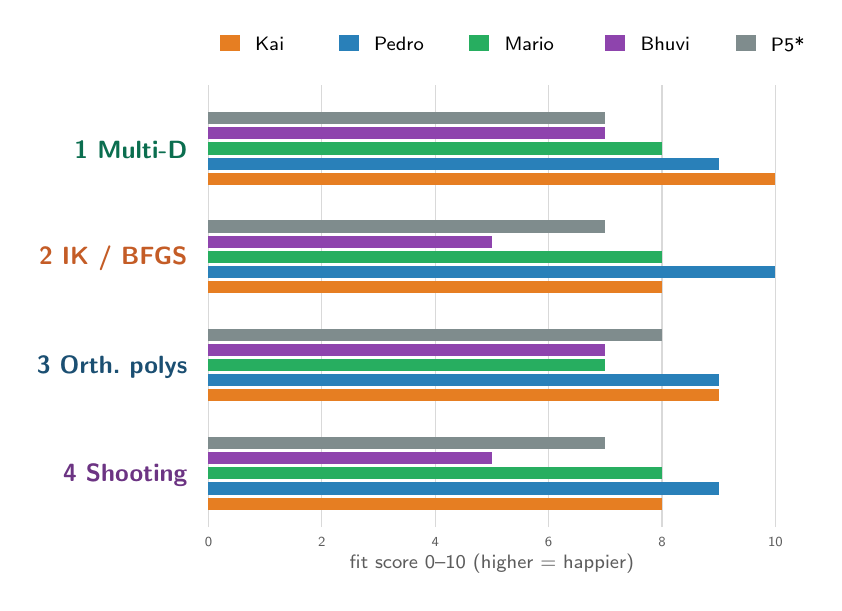
\begin{tikzpicture}[x=0.72cm,y=0.55cm]
  % legend people
  \foreach \name/\col/\x in {Kai/kai/0.2, Pedro/pedro/2.3, Mario/mario/4.6, Bhuvi/bhuvi/7.0, P5*/p5/9.3} {
    \fill[\col] (\x, 11.3) rectangle (\x+0.35, 11.65);
    \node[anchor=west,font=\scriptsize] at (\x+0.45, 11.45) {\name};
  }

  % y labels
  \node[anchor=east,font=\small\bfseries,text=c1] at (-0.2,9) {1 Multi-D};
  \node[anchor=east,font=\small\bfseries,text=c2] at (-0.2,6.5) {2 IK / BFGS};
  \node[anchor=east,font=\small\bfseries,text=c3] at (-0.2,4) {3 Orth.\ polys};
  \node[anchor=east,font=\small\bfseries,text=c4] at (-0.2,1.5) {4 Shooting};

  % grid
  \foreach \x in {0,2,...,10} {
    \draw[line] (\x,0.3) -- (\x,10.5);
    \node[font=\tiny,text=mute] at (\x,-0.05) {\x};
  }

  % bars: proposal y-base, scores
  % 1: 10 9 8 7 7 at y=8.2
  \foreach \i/\s/\col in {0/10/kai,1/9/pedro,2/8/mario,3/7/bhuvi,4/7/p5} {
    \fill[\col] (0, {8.2+0.35*\i}) rectangle (\s, {8.2+0.35*\i+0.28});
  }
  % 2: 8 10 8 5 7
  \foreach \i/\s/\col in {0/8/kai,1/10/pedro,2/8/mario,3/5/bhuvi,4/7/p5} {
    \fill[\col] (0, {5.7+0.35*\i}) rectangle (\s, {5.7+0.35*\i+0.28});
  }
  % 3: 9 9 7 7 8
  \foreach \i/\s/\col in {0/9/kai,1/9/pedro,2/7/mario,3/7/bhuvi,4/8/p5} {
    \fill[\col] (0, {3.2+0.35*\i}) rectangle (\s, {3.2+0.35*\i+0.28});
  }
  % 4: 8 9 8 5 7
  \foreach \i/\s/\col in {0/8/kai,1/9/pedro,2/8/mario,3/5/bhuvi,4/7/p5} {
    \fill[\col] (0, {0.7+0.35*\i}) rectangle (\s, {0.7+0.35*\i+0.28});
  }

  \node[font=\scriptsize,text=mute] at (5,-0.55) {fit score 0--10 (higher = happier)};
\end{tikzpicture}
\end{frame}

%---------------------------------------------------------------------
\begin{frame}{Plain takeaway}
\begin{columns}[T]
\begin{column}{0.48\textwidth}
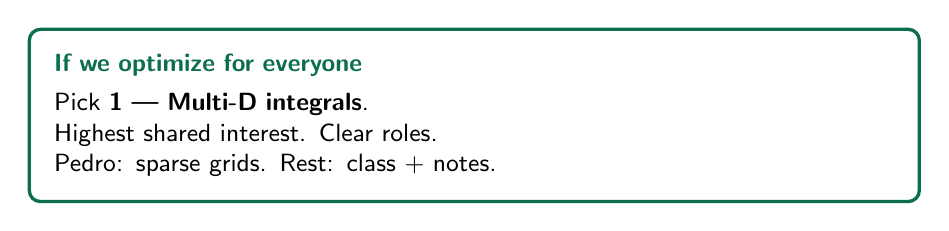
\begin{tikzpicture}
  \node[draw=c1,line width=1.2pt,rounded corners=4pt,align=left,
        font=\small,inner sep=9pt,text width=0.88\textwidth] {
    \textcolor{c1}{\textbf{If we optimize for everyone}}\\[0.35em]
    Pick \textbf{1 --- Multi-D integrals}.\\
    Highest shared interest. Clear roles.\\
    Pedro: sparse grids. Rest: class + notes.
  };
\end{tikzpicture}

\vspace{0.7em}

\begin{tikzpicture}
  \node[draw=c2,line width=1.2pt,rounded corners=4pt,align=left,
        font=\small,inner sep=9pt,text width=0.88\textwidth] {
    \textcolor{c2}{\textbf{If we want the coolest demo}}\\[0.35em]
    Pick \textbf{2 --- Arm aiming (BFGS)}.\\
    Watch Bhuvi's role (demo, not theory).
  };
\end{tikzpicture}
\end{column}
\begin{column}{0.48\textwidth}

\begin{tikzpicture}
  \node[draw=c3,line width=1.2pt,rounded corners=4pt,align=left,
        font=\small,inner sep=9pt,text width=0.88\textwidth] {
    \textcolor{c3}{\textbf{If we want safest oral math}}\\[0.35em]
    Pick \textbf{3 --- Orthogonal polys}.\\
    No weak vetoes. Less flashy app.
  };
\end{tikzpicture}

\vspace{0.7em}
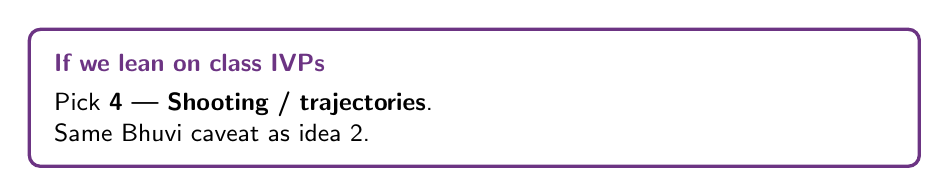
\begin{tikzpicture}
  \node[draw=c4,line width=1.2pt,rounded corners=4pt,align=left,
        font=\small,inner sep=9pt,text width=0.88\textwidth] {
    \textcolor{c4}{\textbf{If we lean on class IVPs}}\\[0.35em]
    Pick \textbf{4 --- Shooting / trajectories}.\\
    Same Bhuvi caveat as idea 2.
  };
\end{tikzpicture}
\end{column}
\end{columns}

\vspace{0.8em}
\centering
{\large\bfseries Next step: each person ranks 1st / 2nd --- then we lock with the instructor.}
\end{frame}

\end{document}
